% Options for packages loaded elsewhere
\PassOptionsToPackage{unicode}{hyperref}
\PassOptionsToPackage{hyphens}{url}
\PassOptionsToPackage{dvipsnames,svgnames,x11names}{xcolor}
%
\documentclass[
  letterpaper,
  DIV=11,
  numbers=noendperiod]{scrreprt}

\usepackage{amsmath,amssymb}
\usepackage{iftex}
\ifPDFTeX
  \usepackage[T1]{fontenc}
  \usepackage[utf8]{inputenc}
  \usepackage{textcomp} % provide euro and other symbols
\else % if luatex or xetex
  \usepackage{unicode-math}
  \defaultfontfeatures{Scale=MatchLowercase}
  \defaultfontfeatures[\rmfamily]{Ligatures=TeX,Scale=1}
\fi
\usepackage{lmodern}
\ifPDFTeX\else  
    % xetex/luatex font selection
\fi
% Use upquote if available, for straight quotes in verbatim environments
\IfFileExists{upquote.sty}{\usepackage{upquote}}{}
\IfFileExists{microtype.sty}{% use microtype if available
  \usepackage[]{microtype}
  \UseMicrotypeSet[protrusion]{basicmath} % disable protrusion for tt fonts
}{}
\makeatletter
\@ifundefined{KOMAClassName}{% if non-KOMA class
  \IfFileExists{parskip.sty}{%
    \usepackage{parskip}
  }{% else
    \setlength{\parindent}{0pt}
    \setlength{\parskip}{6pt plus 2pt minus 1pt}}
}{% if KOMA class
  \KOMAoptions{parskip=half}}
\makeatother
\usepackage{xcolor}
\setlength{\emergencystretch}{3em} % prevent overfull lines
\setcounter{secnumdepth}{-\maxdimen} % remove section numbering
% Make \paragraph and \subparagraph free-standing
\ifx\paragraph\undefined\else
  \let\oldparagraph\paragraph
  \renewcommand{\paragraph}[1]{\oldparagraph{#1}\mbox{}}
\fi
\ifx\subparagraph\undefined\else
  \let\oldsubparagraph\subparagraph
  \renewcommand{\subparagraph}[1]{\oldsubparagraph{#1}\mbox{}}
\fi

\usepackage{color}
\usepackage{fancyvrb}
\newcommand{\VerbBar}{|}
\newcommand{\VERB}{\Verb[commandchars=\\\{\}]}
\DefineVerbatimEnvironment{Highlighting}{Verbatim}{commandchars=\\\{\}}
% Add ',fontsize=\small' for more characters per line
\usepackage{framed}
\definecolor{shadecolor}{RGB}{241,243,245}
\newenvironment{Shaded}{\begin{snugshade}}{\end{snugshade}}
\newcommand{\AlertTok}[1]{\textcolor[rgb]{0.68,0.00,0.00}{#1}}
\newcommand{\AnnotationTok}[1]{\textcolor[rgb]{0.37,0.37,0.37}{#1}}
\newcommand{\AttributeTok}[1]{\textcolor[rgb]{0.40,0.45,0.13}{#1}}
\newcommand{\BaseNTok}[1]{\textcolor[rgb]{0.68,0.00,0.00}{#1}}
\newcommand{\BuiltInTok}[1]{\textcolor[rgb]{0.00,0.23,0.31}{#1}}
\newcommand{\CharTok}[1]{\textcolor[rgb]{0.13,0.47,0.30}{#1}}
\newcommand{\CommentTok}[1]{\textcolor[rgb]{0.37,0.37,0.37}{#1}}
\newcommand{\CommentVarTok}[1]{\textcolor[rgb]{0.37,0.37,0.37}{\textit{#1}}}
\newcommand{\ConstantTok}[1]{\textcolor[rgb]{0.56,0.35,0.01}{#1}}
\newcommand{\ControlFlowTok}[1]{\textcolor[rgb]{0.00,0.23,0.31}{#1}}
\newcommand{\DataTypeTok}[1]{\textcolor[rgb]{0.68,0.00,0.00}{#1}}
\newcommand{\DecValTok}[1]{\textcolor[rgb]{0.68,0.00,0.00}{#1}}
\newcommand{\DocumentationTok}[1]{\textcolor[rgb]{0.37,0.37,0.37}{\textit{#1}}}
\newcommand{\ErrorTok}[1]{\textcolor[rgb]{0.68,0.00,0.00}{#1}}
\newcommand{\ExtensionTok}[1]{\textcolor[rgb]{0.00,0.23,0.31}{#1}}
\newcommand{\FloatTok}[1]{\textcolor[rgb]{0.68,0.00,0.00}{#1}}
\newcommand{\FunctionTok}[1]{\textcolor[rgb]{0.28,0.35,0.67}{#1}}
\newcommand{\ImportTok}[1]{\textcolor[rgb]{0.00,0.46,0.62}{#1}}
\newcommand{\InformationTok}[1]{\textcolor[rgb]{0.37,0.37,0.37}{#1}}
\newcommand{\KeywordTok}[1]{\textcolor[rgb]{0.00,0.23,0.31}{#1}}
\newcommand{\NormalTok}[1]{\textcolor[rgb]{0.00,0.23,0.31}{#1}}
\newcommand{\OperatorTok}[1]{\textcolor[rgb]{0.37,0.37,0.37}{#1}}
\newcommand{\OtherTok}[1]{\textcolor[rgb]{0.00,0.23,0.31}{#1}}
\newcommand{\PreprocessorTok}[1]{\textcolor[rgb]{0.68,0.00,0.00}{#1}}
\newcommand{\RegionMarkerTok}[1]{\textcolor[rgb]{0.00,0.23,0.31}{#1}}
\newcommand{\SpecialCharTok}[1]{\textcolor[rgb]{0.37,0.37,0.37}{#1}}
\newcommand{\SpecialStringTok}[1]{\textcolor[rgb]{0.13,0.47,0.30}{#1}}
\newcommand{\StringTok}[1]{\textcolor[rgb]{0.13,0.47,0.30}{#1}}
\newcommand{\VariableTok}[1]{\textcolor[rgb]{0.07,0.07,0.07}{#1}}
\newcommand{\VerbatimStringTok}[1]{\textcolor[rgb]{0.13,0.47,0.30}{#1}}
\newcommand{\WarningTok}[1]{\textcolor[rgb]{0.37,0.37,0.37}{\textit{#1}}}

\providecommand{\tightlist}{%
  \setlength{\itemsep}{0pt}\setlength{\parskip}{0pt}}\usepackage{longtable,booktabs,array}
\usepackage{calc} % for calculating minipage widths
% Correct order of tables after \paragraph or \subparagraph
\usepackage{etoolbox}
\makeatletter
\patchcmd\longtable{\par}{\if@noskipsec\mbox{}\fi\par}{}{}
\makeatother
% Allow footnotes in longtable head/foot
\IfFileExists{footnotehyper.sty}{\usepackage{footnotehyper}}{\usepackage{footnote}}
\makesavenoteenv{longtable}
\usepackage{graphicx}
\makeatletter
\def\maxwidth{\ifdim\Gin@nat@width>\linewidth\linewidth\else\Gin@nat@width\fi}
\def\maxheight{\ifdim\Gin@nat@height>\textheight\textheight\else\Gin@nat@height\fi}
\makeatother
% Scale images if necessary, so that they will not overflow the page
% margins by default, and it is still possible to overwrite the defaults
% using explicit options in \includegraphics[width, height, ...]{}
\setkeys{Gin}{width=\maxwidth,height=\maxheight,keepaspectratio}
% Set default figure placement to htbp
\makeatletter
\def\fps@figure{htbp}
\makeatother

\KOMAoption{captions}{tableheading}
\makeatletter
\makeatother
\makeatletter
\makeatother
\makeatletter
\@ifpackageloaded{caption}{}{\usepackage{caption}}
\AtBeginDocument{%
\ifdefined\contentsname
  \renewcommand*\contentsname{Table of contents}
\else
  \newcommand\contentsname{Table of contents}
\fi
\ifdefined\listfigurename
  \renewcommand*\listfigurename{List of Figures}
\else
  \newcommand\listfigurename{List of Figures}
\fi
\ifdefined\listtablename
  \renewcommand*\listtablename{List of Tables}
\else
  \newcommand\listtablename{List of Tables}
\fi
\ifdefined\figurename
  \renewcommand*\figurename{Figure}
\else
  \newcommand\figurename{Figure}
\fi
\ifdefined\tablename
  \renewcommand*\tablename{Table}
\else
  \newcommand\tablename{Table}
\fi
}
\@ifpackageloaded{float}{}{\usepackage{float}}
\floatstyle{ruled}
\@ifundefined{c@chapter}{\newfloat{codelisting}{h}{lop}}{\newfloat{codelisting}{h}{lop}[chapter]}
\floatname{codelisting}{Listing}
\newcommand*\listoflistings{\listof{codelisting}{List of Listings}}
\makeatother
\makeatletter
\@ifpackageloaded{caption}{}{\usepackage{caption}}
\@ifpackageloaded{subcaption}{}{\usepackage{subcaption}}
\makeatother
\makeatletter
\@ifpackageloaded{tcolorbox}{}{\usepackage[skins,breakable]{tcolorbox}}
\makeatother
\makeatletter
\@ifundefined{shadecolor}{\definecolor{shadecolor}{rgb}{.97, .97, .97}}
\makeatother
\makeatletter
\makeatother
\makeatletter
\makeatother
\ifLuaTeX
  \usepackage{selnolig}  % disable illegal ligatures
\fi
\IfFileExists{bookmark.sty}{\usepackage{bookmark}}{\usepackage{hyperref}}
\IfFileExists{xurl.sty}{\usepackage{xurl}}{} % add URL line breaks if available
\urlstyle{same} % disable monospaced font for URLs
\hypersetup{
  pdftitle={Week3-Exercises-Solutions},
  colorlinks=true,
  linkcolor={blue},
  filecolor={Maroon},
  citecolor={Blue},
  urlcolor={Blue},
  pdfcreator={LaTeX via pandoc}}

\title{Week3-Exercises-Solutions}
\author{}
\date{}

\begin{document}
\maketitle
\ifdefined\Shaded\renewenvironment{Shaded}{\begin{tcolorbox}[boxrule=0pt, sharp corners, enhanced, breakable, frame hidden, interior hidden, borderline west={3pt}{0pt}{shadecolor}]}{\end{tcolorbox}}\fi

\hypertarget{exercise-solutions}{%
\chapter{Exercise solutions}\label{exercise-solutions}}

\hypertarget{week-3}{%
\subsection*{Week 3}\label{week-3}}
\addcontentsline{toc}{subsection}{Week 3}

The dataset
\href{https://www.dropbox.com/scl/fi/ljqh7xojwidza0h1e7lg4/lowbwt.csv?rlkey=stg6s90y1aqr4eo9pkxkm73bl\&dl=1}{lowbwt.csv}
was part of a study aiming to identify risk factors associated with
giving birth to a low birth weight baby (weighing less than 2500 grams).

\hypertarget{fit-a-linear-model-for-the-variable-bwt-birth-weight-using-the-covariate-age-mothers-age-evaluate-the-assumptions-and-interpret-the-results.}{%
\subsubsection{\texorpdfstring{1 - Fit a linear model for the variable
\emph{bwt} (birth weight) using the covariate \emph{age} (mother's age),
evaluate the assumptions and interpret the
results.}{1 - Fit a linear model for the variable bwt (birth weight) using the covariate age (mother's age), evaluate the assumptions and interpret the results.}}\label{fit-a-linear-model-for-the-variable-bwt-birth-weight-using-the-covariate-age-mothers-age-evaluate-the-assumptions-and-interpret-the-results.}}

\textbf{R code}

\begin{Shaded}
\begin{Highlighting}[]
\NormalTok{lowbwt }\OtherTok{\textless{}{-}} \FunctionTok{read.csv}\NormalTok{(}\StringTok{"https://www.dropbox.com/scl/fi/ljqh7xojwidza0h1e7lg4/lowbwt.csv?rlkey=stg6s90y1aqr4eo9pkxkm73bl\&dl=1"}\NormalTok{)   }
\NormalTok{lm1 }\OtherTok{\textless{}{-}} \FunctionTok{lm}\NormalTok{(bwt}\SpecialCharTok{\textasciitilde{}}\NormalTok{age, }\AttributeTok{data=}\NormalTok{lowbwt)  }\CommentTok{\#fit  the model}
\FunctionTok{summary}\NormalTok{(lm1)}
\end{Highlighting}
\end{Shaded}

\begin{verbatim}

Call:
lm(formula = bwt ~ age, data = lowbwt)

Residuals:
     Min       1Q   Median       3Q      Max 
-2294.53  -517.71    10.56   530.65  1776.27 

Coefficients:
            Estimate Std. Error t value Pr(>|t|)    
(Intercept)  2657.33     238.80  11.128   <2e-16 ***
age            12.36      10.02   1.234    0.219    
---
Signif. codes:  0 '***' 0.001 '**' 0.01 '*' 0.05 '.' 0.1 ' ' 1

Residual standard error: 728 on 187 degrees of freedom
Multiple R-squared:  0.008076,  Adjusted R-squared:  0.002772 
F-statistic: 1.523 on 1 and 187 DF,  p-value: 0.2188
\end{verbatim}

\begin{Shaded}
\begin{Highlighting}[]
\FunctionTok{confint}\NormalTok{(lm1)}
\end{Highlighting}
\end{Shaded}

\begin{verbatim}
                  2.5 %     97.5 %
(Intercept) 2186.236438 3128.42869
age           -7.403527   32.13219
\end{verbatim}

\begin{Shaded}
\begin{Highlighting}[]
\FunctionTok{par}\NormalTok{(}\AttributeTok{mfrow=}\FunctionTok{c}\NormalTok{(}\DecValTok{1}\NormalTok{,}\DecValTok{2}\NormalTok{))}
\FunctionTok{plot}\NormalTok{(lm1, }\FunctionTok{c}\NormalTok{(}\DecValTok{1}\NormalTok{,}\DecValTok{2}\NormalTok{)) }\CommentTok{\#residuals vs fitted and distrib of the residuals}
\end{Highlighting}
\end{Shaded}

\begin{figure}[H]

{\centering 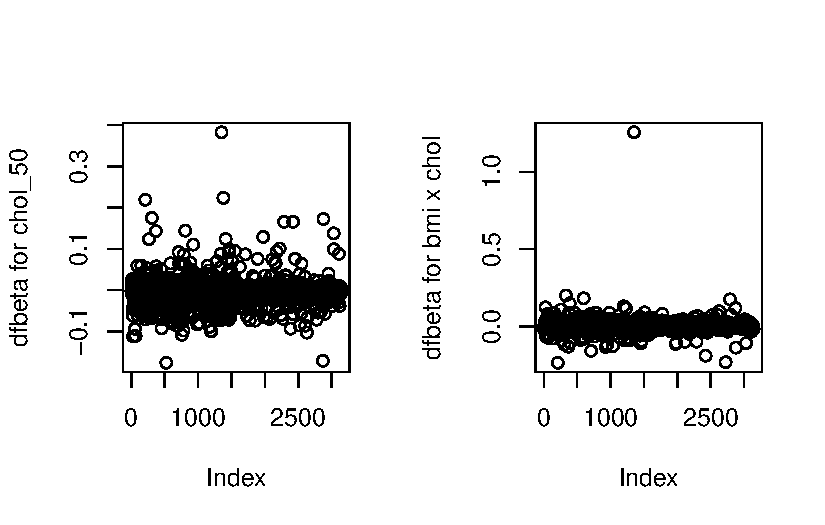
\includegraphics{Week3_exerc_sol_files/figure-pdf/unnamed-chunk-1-1.pdf}

}

\end{figure}

\textbf{Stata code}

\begin{Shaded}
\begin{Highlighting}[]
\KeywordTok{clear}
\NormalTok{import delimited }\StringTok{"https://www.dropbox.com/scl/fi/ljqh7xojwidza0h1e7lg4/lowbwt.csv?rlkey=stg6s90y1aqr4eo9pkxkm73bl\&dl=1"}

\KeywordTok{reg}\NormalTok{ bwt age}
\KeywordTok{rvfplot} 
\KeywordTok{predict}\NormalTok{ res\_std, residuals }\CommentTok{/* calculate the residuals*/}
\KeywordTok{qnorm}\NormalTok{ res\_std }\CommentTok{/* The normal quantile plot of the residuals*/}
\NormalTok{\#\# (encoding automatically selected: UTF{-}8)}
\NormalTok{\#\# (11 vars, 189 }\KeywordTok{obs}\NormalTok{)}
\NormalTok{\#\# }
\NormalTok{\#\# }
\NormalTok{\#\#       Source |       SS           df       MS      Number }\KeywordTok{of} \KeywordTok{obs}\NormalTok{   =       189}
\NormalTok{\#\# {-}{-}{-}{-}{-}{-}{-}{-}{-}{-}{-}{-}{-}+{-}{-}{-}{-}{-}{-}{-}{-}{-}{-}{-}{-}{-}{-}{-}{-}{-}{-}{-}{-}{-}{-}{-}{-}{-}{-}{-}{-}{-}{-}{-}{-}{-}{-}   }\FunctionTok{F}\NormalTok{(1, 187)       =      1.52}
\NormalTok{\#\#        Model |  806926.913         1  806926.913   Prob \textgreater{} }\FunctionTok{F}\NormalTok{        =    0.2188}
\NormalTok{\#\#     Residual |  99110125.7       187  530000.672   R{-}squared       =    0.0081}
\NormalTok{\#\# {-}{-}{-}{-}{-}{-}{-}{-}{-}{-}{-}{-}{-}+{-}{-}{-}{-}{-}{-}{-}{-}{-}{-}{-}{-}{-}{-}{-}{-}{-}{-}{-}{-}{-}{-}{-}{-}{-}{-}{-}{-}{-}{-}{-}{-}{-}{-}   Adj R{-}squared   =    0.0028}
\NormalTok{\#\#        Total |  99917052.6       188  531473.684   Root MSE        =    728.01}
\NormalTok{\#\# }
\NormalTok{\#\# {-}{-}{-}{-}{-}{-}{-}{-}{-}{-}{-}{-}{-}{-}{-}{-}{-}{-}{-}{-}{-}{-}{-}{-}{-}{-}{-}{-}{-}{-}{-}{-}{-}{-}{-}{-}{-}{-}{-}{-}{-}{-}{-}{-}{-}{-}{-}{-}{-}{-}{-}{-}{-}{-}{-}{-}{-}{-}{-}{-}{-}{-}{-}{-}{-}{-}{-}{-}{-}{-}{-}{-}{-}{-}{-}{-}{-}{-}}
\NormalTok{\#\#          bwt | Coefficient  Std. err.      t    P\textgreater{}|t|     [95\% conf. interval]}
\NormalTok{\#\# {-}{-}{-}{-}{-}{-}{-}{-}{-}{-}{-}{-}{-}+{-}{-}{-}{-}{-}{-}{-}{-}{-}{-}{-}{-}{-}{-}{-}{-}{-}{-}{-}{-}{-}{-}{-}{-}{-}{-}{-}{-}{-}{-}{-}{-}{-}{-}{-}{-}{-}{-}{-}{-}{-}{-}{-}{-}{-}{-}{-}{-}{-}{-}{-}{-}{-}{-}{-}{-}{-}{-}{-}{-}{-}{-}{-}{-}}
\NormalTok{\#\#          age |   12.36433   10.02055     1.23   0.219    {-}7.403527    32.13219}
\NormalTok{\#\#        }\DataTypeTok{\_cons}\NormalTok{ |   2657.333    238.804    11.13   0.000     2186.236    3128.429}
\NormalTok{\#\# {-}{-}{-}{-}{-}{-}{-}{-}{-}{-}{-}{-}{-}{-}{-}{-}{-}{-}{-}{-}{-}{-}{-}{-}{-}{-}{-}{-}{-}{-}{-}{-}{-}{-}{-}{-}{-}{-}{-}{-}{-}{-}{-}{-}{-}{-}{-}{-}{-}{-}{-}{-}{-}{-}{-}{-}{-}{-}{-}{-}{-}{-}{-}{-}{-}{-}{-}{-}{-}{-}{-}{-}{-}{-}{-}{-}{-}{-}}
\end{Highlighting}
\end{Shaded}

We have fitted a linear regression for birth weight using mother's age.
The first residual plot (residuals vs fitted) does not show evidence of
departure from the linearity assumption or violation of the
homoscedasticity assumption as the dispersion seems constant along the
x-axis. The q-q plot indicates that the residuals appear to follow a
normal distribution (a bit of departure at one of the tails).

From the regression output, the intercept 2657, which is the expected
birth weight for a mother with an age of zero. The coefficient for age
is 12, which means that for every one year increase in the mother's age,
the birth weight is expected to increase 12 grams in average (95\%CI:
{[}-7, 32{]}). The R-squared value for this model is 0.008. This means
that 0.8\% of the variability in birth weight can be explained by the
mother's age. This result does not provide evidence of a linear relation
between birth weight and mother's age.

\hypertarget{evaluate-potential-outliers-and-influential-observations.-how-would-the-results-change-if-you-excluded-thisthese-observations}{%
\subsubsection{2 - Evaluate potential outliers and influential
observations. How would the results change if you excluded this/these
observation(s)?}\label{evaluate-potential-outliers-and-influential-observations.-how-would-the-results-change-if-you-excluded-thisthese-observations}}

\begin{Shaded}
\begin{Highlighting}[]
\FunctionTok{plot}\NormalTok{(lowbwt}\SpecialCharTok{$}\NormalTok{age, lowbwt}\SpecialCharTok{$}\NormalTok{bwt)}
\FunctionTok{text}\NormalTok{(lowbwt}\SpecialCharTok{$}\NormalTok{age, lowbwt}\SpecialCharTok{$}\NormalTok{bwt, }\AttributeTok{labels =}\NormalTok{ lowbwt}\SpecialCharTok{$}\NormalTok{id, }\AttributeTok{pos =} \DecValTok{1}\NormalTok{) }\CommentTok{\#adds ids}
\end{Highlighting}
\end{Shaded}

\begin{figure}[H]

{\centering 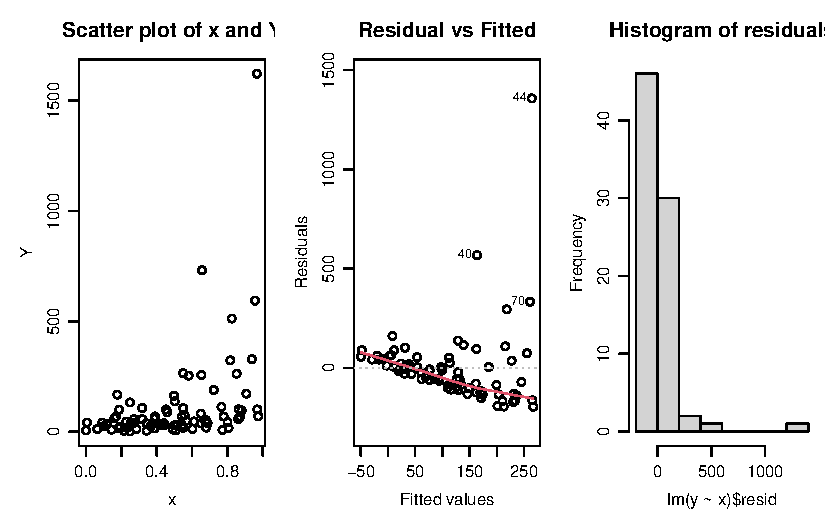
\includegraphics{Week3_exerc_sol_files/figure-pdf/unnamed-chunk-3-1.pdf}

}

\end{figure}

From the scatter plot, we can recognise the observation with id=226 has
a value for age far from the other observations. Let's look at some
plots with influence measures:

\begin{Shaded}
\begin{Highlighting}[]
\CommentTok{\#Cook\textquotesingle{}s distance}
\CommentTok{\#the option labels.id shows the label from }
\CommentTok{\#the variable id rather than the row number}
\FunctionTok{plot}\NormalTok{(lm1, }\FunctionTok{c}\NormalTok{(}\DecValTok{4}\NormalTok{,}\DecValTok{5}\NormalTok{), }\AttributeTok{labels.id=}\NormalTok{lowbwt}\SpecialCharTok{$}\NormalTok{id)  }
\end{Highlighting}
\end{Shaded}

\begin{figure}[H]

{\centering 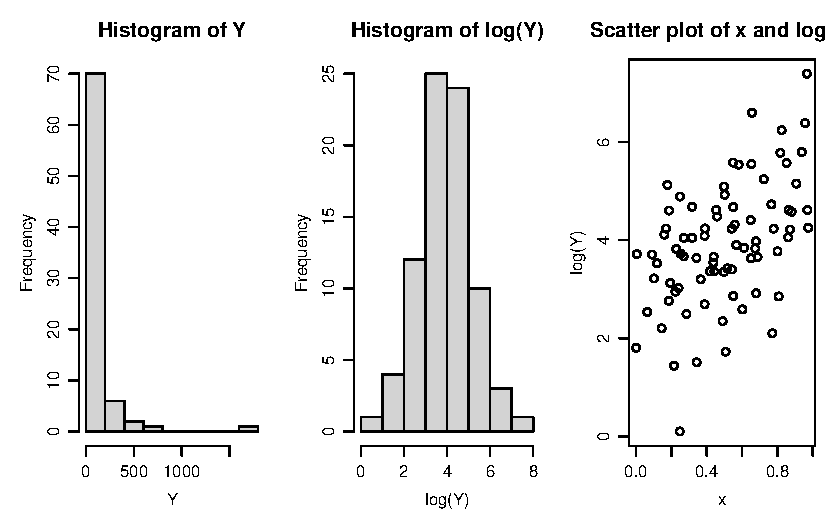
\includegraphics{Week3_exerc_sol_files/figure-pdf/unnamed-chunk-4-1.pdf}

}

\end{figure}

\begin{figure}[H]

{\centering \includegraphics{Week3_exerc_sol_files/figure-pdf/unnamed-chunk-4-2.pdf}

}

\end{figure}

\begin{Shaded}
\begin{Highlighting}[]
\CommentTok{\#Plotting the change in the beta for age}
\CommentTok{\#when each observation is removed}
\NormalTok{inf }\OtherTok{\textless{}{-}} \FunctionTok{influence.measures}\NormalTok{(lm1)}
\FunctionTok{plot}\NormalTok{(lowbwt}\SpecialCharTok{$}\NormalTok{id, inf}\SpecialCharTok{$}\NormalTok{infmat[,}\DecValTok{2}\NormalTok{], }\AttributeTok{xlab=}\StringTok{"ID"}\NormalTok{, }\AttributeTok{ylab=}\StringTok{"mother\textquotesingle{}s age"}\NormalTok{)}
\FunctionTok{text}\NormalTok{(lowbwt}\SpecialCharTok{$}\NormalTok{id, inf}\SpecialCharTok{$}\NormalTok{infmat[,}\DecValTok{2}\NormalTok{], }\AttributeTok{labels =}\NormalTok{ lowbwt}\SpecialCharTok{$}\NormalTok{id, }\AttributeTok{pos =} \DecValTok{1}\NormalTok{, }\AttributeTok{cex=}\NormalTok{.}\DecValTok{7}\NormalTok{) }\CommentTok{\#adds ids}
\FunctionTok{title}\NormalTok{(}\StringTok{"beta\_age with ID removed"}\NormalTok{)}
\end{Highlighting}
\end{Shaded}

\begin{figure}[H]

{\centering \includegraphics{Week3_exerc_sol_files/figure-pdf/unnamed-chunk-4-3.pdf}

}

\end{figure}

\begin{Shaded}
\begin{Highlighting}[]
\KeywordTok{clear}
\NormalTok{import delimited }\StringTok{"https://www.dropbox.com/s/r06u1l1cjrvcpl1/lowbwt.csv?dl=1"}
\KeywordTok{reg}\NormalTok{ bwt age}
\KeywordTok{dfbeta}
\CommentTok{/*leverage plot /*}
\CommentTok{lvr2plot }

\CommentTok{/*plotting the change in the beta for age  (dfbeta) }
\CommentTok{when each observation is removed/*}
\CommentTok{twoway (scatter \_dfbeta\_1 id, sort mlabel(id))}
\CommentTok{\#\# server refused to send file}
\CommentTok{\#\# could not open url}
\CommentTok{\#\# r(603);}
\CommentTok{\#\# }
\CommentTok{\#\# r(603);}
\end{Highlighting}
\end{Shaded}

After reviewing the plots above, it appears that both observation 11 and
226 have a significant impact on the estimation. As a general rule, it
is not advisable to remove observations from the analysis without a
strong justification, and any such decision should be well-justified.
However, in this instance, observation 226 was made on a mother who is
nearly 10 years older than the older mothers in the remaining cohort.
This factor may suggest that this mother belongs to a different cohort,
and we could argue for her exclusion from the analysis. Regardless, it
would have been preferable to anticipate this issue during the study's
design phase, for instance, by setting age\textless40 years old as an
inclusion criterion.



\end{document}
